% Required libraries
\documentclass[9pt]{llncs}
\usepackage{llncsdoc}
\usepackage{graphicx}
%\usepackage{float}
%\usepackage{cite}
\usepackage{lipsum}
\usepackage{mwe}
\usepackage{hyperref} 
\usepackage{fixltx2e}
\usepackage{wrapfig}
\usepackage{subfig}
%\usepackage{natbib}
%\usepackage{mwe}
%\usepackage{cleveref}
%\usepackage{titlesec}
%\usepackage{fixfoot}
\newcommand{\beginsupplement}{%
        \setcounter{table}{0}
        \renewcommand{\thetable}{S\arabic{table}}%
        \setcounter{figure}{0}
        \renewcommand{\thefigure}{S\arabic{figure}}%
     }

% The package uses instructions from Springer (http://www.springer.com/gp/computer-science/lncs/conference-proceedings-guidelines)
% Instructions.tex contains the doc file with documentation etc
% Also available in this link (https://www.overleaf.com/9039312xjbbvqpqdkrk) to see it as another LaTeX document

% Instructions for images, figures and refs are at the end of the document


%%%%%%%%%%%%%%%%%%%%%%%%%%%%%%%%%
% Process report --> https://www.overleaf.com/9678422wqkxxqywnwpc 
%%%%%%%%%%%%%%%%%%%%%%%%%%%%%%%%%

\begin{document}
\title{Predicting hotel preferences from user query search}%??
\author{Marie Corradi (2596976)\inst{1}, Elena Garcia (2604289) \inst{1}, Alberto Gil (2595259)\inst{1}}
\institute{MSc Bioinformatics and Systems Biology. Vrije University Amsterdam}
\maketitle

%%%% INTRODUCTION %%%%%%%%%%%
Hotel booking and travel websites are one of the most prominent business of the moment. Expedia, for instance, had a net income of 281.8 million in 2016 \cite{2017ExpediaResults}. 
The major advantage that companies like Expedia can benefit from is the huge amount of data stored in their data centers. Data driven decisions could have a major impact in the company's revenue if Big Data is handled properly. Nevertheless, this requires highly sophisticated data preprocessing and complex algorithms.


With this motivation, Expedia has launched to date two Kaggle competitions with the 
"Personalize Expedia Hotel Searches - ICDM 2013" \cite{ExpediaHttps://www.kaggle.com/c/expedia-personalized-sort} and in 2016 "Expedia Hotel Recommendations" \cite{ExpediaHttps://www.kaggle.com/c/expedia-hotel-recommendations}.


This project is based on the the 2013 Expedia Kaggle competition. The dataset used was released by Expedia with the aim of improving their ranking on hotel searches. The main objective towards this challenge is facing the ranking problem of Machine Learning \cite{Liu2007LearningRetrieval} in an objective and creative way, as the goal is to create a model able to rank hotels according to the likeliness to be booked. 

%Learning to rank[1] or machine-learned ranking (MLR) is the application of machine learning, typically supervised, semi-supervised or reinforcement learning, in the construction of ranking models for information retrieval systems.[2] Training data consists of lists of items with some partial order specified between items in each list. This order is typically induced by giving a numerical or ordinal score or a binary judgment (e.g. "relevant" or "not relevant") for each item. The ranking model's purpose is to rank, i.e. produce a permutation of items in new, unseen lists in a way which is "similar" to rankings in the training data in some sense.

%%%%%%% Business understanding %%%%%%%%%%%
\section{Business understanding}
The Kaggle 2013 competitions winners released several (potentially) useful descriptions about their approaches \cite{ExpediaHttps://www.kaggle.com/c/expedia-personalized-sort/discussion/6203}. 


In Kaggle forum \cite{ExpediaHttps://www.kaggle.com/c/expedia-personalized-sort} several people used Extreme Gradient Boosting (XGBoost), which is based on Gradient Boosting \cite{XGB}. 
%http://xgboost.readthedocs.io/en/latest/model.html

We had a look at the 2016's Expedia competition winner's topic \cite{Kaggle21607}.
%https://www.kaggle.com/c/expedia-hotel-recommendations/discussion/21607

Some tips about how to handle this dataset can be found at Dataquest \cite{Parachuri}.
%https://www.dataquest.io/blog/kaggle-tutorial/

Another approach that we found was in \cite{AgarwalLearnQueries}, in which a separate Random Forest for every country\_id was built yielding a NDCG score of 0.51.
However, not only the algorithms were discussed, but the importance of feature pre-processing and engineering was also highlighted, with some of the top competitors having engineered over 300 features in addition to the ones initially given by Expedia.

\section{Data Exploration}
The original dataset was formed by a random selection from Expedia web-page \cite{ExpediaHttps://www.kaggle.com/c/expedia-personalized-sort}, formed by 4.958.348 rows containing information shown on hotel's searches. Around 400.000 different searches comprised this dataset, having information from 129.113 different hotels, and 199.795 different searches (matching in average 25 hotels shown per search). 
\subsection{Overall exploration}
For the data exploration, we used the format pandas data frame \cite{McKinney2015PandasToolkit}. In order to make a better use of the date information, we transformed the column in two: 'year' and 'month'.
We then plotted the distributions of the different variables (script data\_exploration.py). The graphics (not shown) shows that the distribution of the values in the general features follows a normal distribution in numerical variables and uniform when variables are discrete.


In more detail, visitor\_location\_country\_id has one location (country ID 219) that is the most abundant significantly, although srch\_destination\_id is similar across all IDs. Other interesting information is that the users search the most for 1 room and below 4 days. The majority of the searches are done for 2 adults and no children. The most common month booked is June (calculated using a new variable month\_booked). And mostly there was no promotion flag.


\subsection{Variables correlation}
According to the winners of the Expedia competition in 2013, 
prop\_starrating and prop\_review\_score are positively correlated, and there are strong (anti-)correlations between variables of hotel characteristics \cite{ExpediaHttps://www.kaggle.com/c/expedia-personalized-sort/discussion/6203}.


As observed in the heatmap[\ref{heatmap}], several variables are strongly correlated (either positively or negatively). None of the variables has such a strong correlation that we considered removing them because of redundancy.

\begin{figure}%{0.5\textwidth}
\centering
	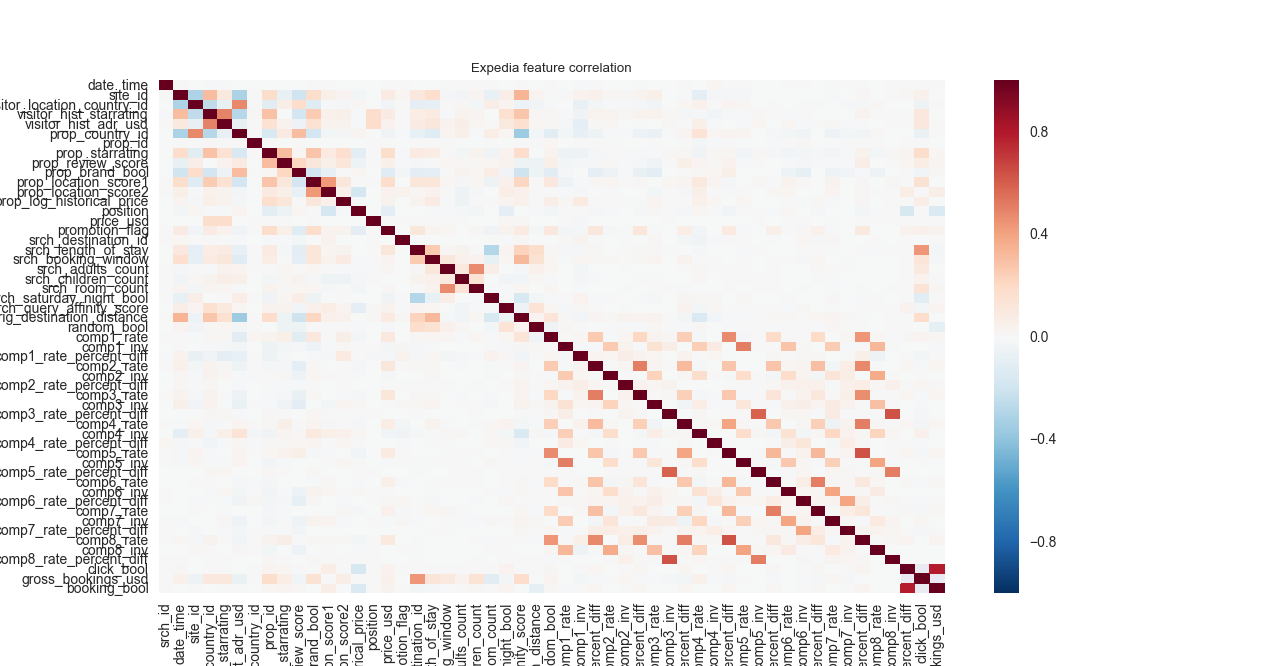
\includegraphics[width=0.7\textwidth]{feature_correlation_whole_dataset.png}
	\caption{Heatmap of all-against-all variables. }
    \label{heatmap}
\end{figure}

\subsection{Effect of missing information of a query}
Several variables lack of information in the dataset.
There are variables with >90\% missing data (specifically the visitor’s historical data (ratings, shops),  the competitors information, the search query affinity score and the gross booking spent).
Most of the search\_id have 40-60\% of the data missing.
Around 32\% of the rows representing a hotel booked are missing information from orig\_destination\_distance.
We observed how the lack of information of certain variables translated into a lower probability of a hotel being booked [\ref{mp_1a}, \ref{mp_1b}].

\begin{figure}[h]
     \centering
     \begin{minipage}{0.45\textwidth}
     \centering
     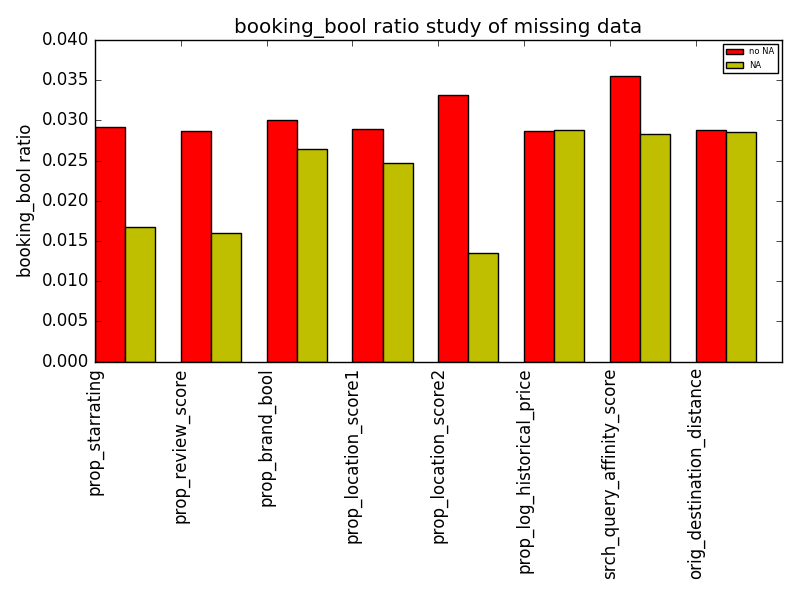
\includegraphics[width=0.9\textwidth]{missing_info_booking_bool_ratio.png}
         \caption{Percentage of bookings that occur, when certain variables have missing values. }
         \label{mp_1a}
     \end{minipage}\hfill
     \begin{minipage}{0.45\textwidth}
         \centering
         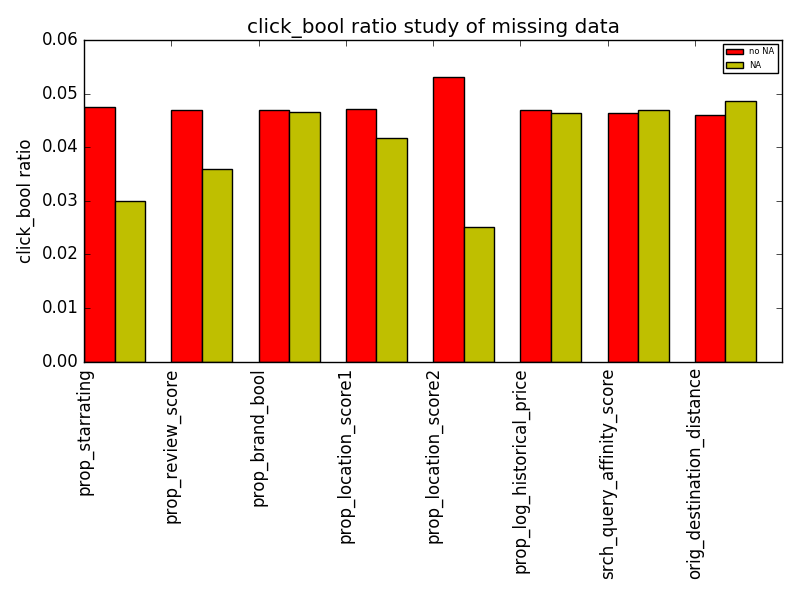
\includegraphics[width=0.9\textwidth]{missing_info_click_bool_ratio.png}
         \caption{Percentage of clicks that occur, when certain variables have missing values.}
         \label{mp_1b}
     \end{minipage}
\end{figure}


It is clear from the previous plot that prop\_starrating, prop\_review\_score and prop\_location\_score2 have an impact on the user behavior when there is missing information.



%This can be seen in more detail in [\ref{table_mp}].
%\begin{table}
%\tiny
%\centering
%\caption{Percentage of missing points per variable.}
%\begin{tabular}{lllllll}
%\hline\noalign{\smallskip}
%\textbf{Variable} & \textbf{\% Missing points} \\
%\noalign{\smallskip}
%\hline
%\noalign{\smallskip}
%visitor\_hist\_starrating & 94\% \\
%Visitor\_hist\_adr\_usd& 95\%\\
%prop\_review\_score & 0.2\%\\ 
%prop\_location\_score\_2 & 22\% \\ 
%srch\_query\_affinity\_score & 94\% \\
%orig\_destination\_distance & 32\% \\
%gross\_bookings\_usd  & 97\%\\
%month\_book & months since the first time record
%scores\_merged& aa\\
%comp1\_rate, comp1\_inv, comp1\_rate\_percent\_diff & 98\% \\
%comp2\_rate, comp2\_inv & 59\%\\ 
%comp2\_rate\_percent\_diff &59\% \\
%comp3\_rate, comp3\_inv & 69\%\\ 
%comp3\_rate\_percent\_diff &90\% \\
%comp4\_rate, comp4\_inv & 93\%\\ 
%comp4\_rate\_percent\_diff &97\% \\
%comp5\_rate, comp5\_inv & 55\%\\ 
%comp5\_rate\_percent\_diff &83\% \\
%comp6\_rate, comp6\_inv & 95\%\\ 
%comp6\_rate\_percent\_diff &98\% \\
%comp7\_rate, comp7\_inv & 93\%\\ 
%comp7\_rate\_percent\_diff &97\% \\
%comp8\_rate, comp8\_inv & 95\%\\ 
%comp8\_rate\_percent\_diff &87\% \\
%\hline
%\end{tabular}
%\label{table_mp}
%\end{table}


\subsection{Outliers}
We then searched for obvious outliers that would spoil the models’ performance. Very few searches had price\_usd bigger than \$5.000 (figure not shown). Expedia is a platform where we would not expect clients to spend that amount of money, so we decided to delete those searches.

\subsection{Dominance of negative data in the dataset}
In the full training set, we found that 61405 srch\_ID have never booked a hotel on their search, whereas 138390 srch\_id have booked a hotel. Nevertheless, taking into account the total number of rows, only 2,8\% of the original dataset had information about a hotel being booked. Clearly, the dataset is biased towards the presence of negative data.

\subsection{Bias in booking and clicking}
We found a strong position bias even for random impressions [\ref{mp_2a},\ref{mp_2b} \ref{table_bias}]. The position of the listed hotels has a great impact on the booking counts, but not so on the clicking events. 

\begin{figure}[h]
     \centering
     \begin{minipage}{0.45\textwidth}
     \centering
     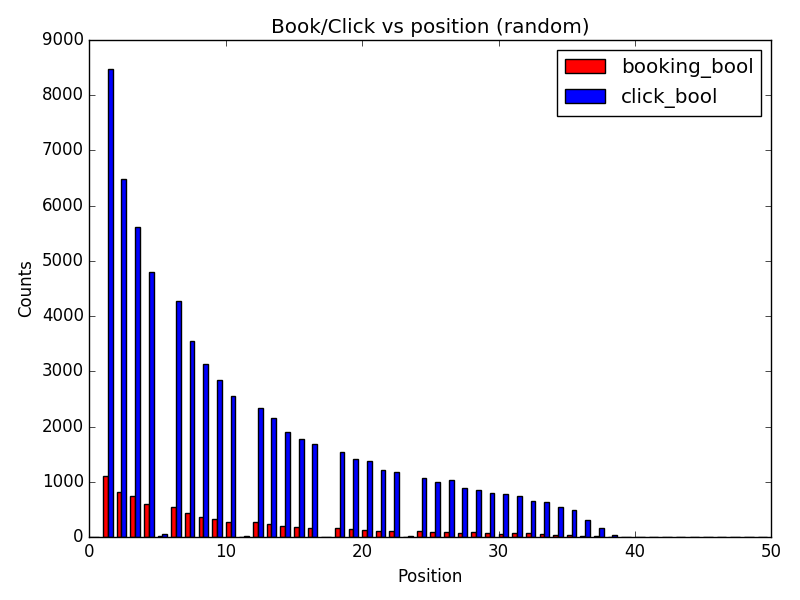
\includegraphics[width=0.9\textwidth]{hotel_position_vs_click_booking_random.png}
         \caption{Position order of the hotels affects the booking number, but not the clicking.}
         \label{mp_2a}
     \end{minipage}\hfill
     \begin{minipage}{0.45\textwidth}
         \centering
         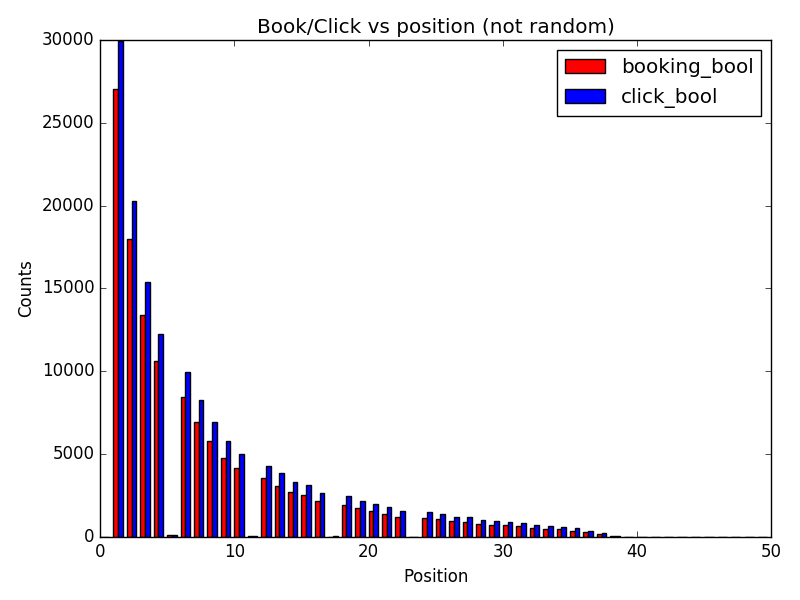
\includegraphics[width=0.9\textwidth]{hotel_position_vs_click_booking_notrandom.png}
         \caption{There is a strong bias in the position and the booking.}
         \label{mp_2b}
     \end{minipage}
 \end{figure}
%%%%%%%%%%%%%%%%%%%%
\begin{table}
\tiny
\centering
\caption{Bias.}
\begin{tabular}{lllllll}
\hline\noalign{\smallskip}
\textbf{} & \textbf{Random = 1} & \textbf{Random = 0}  & \textbf{Total} \\
\noalign{\smallskip}
\hline
\noalign{\smallskip}
\% book/click & 11.4\% & 85.1\% & 2.8\%\\
\% book/total & 0.5\% & 3.7\% & 2.8\%\\
\% click/total & 4.7\% & 4.4\% & 4.5\%\\
\hline
\end{tabular}
\label{table_bias}
\end{table}


\section{Data Preprocessing}
\subsection{Missing points}
In the course of the data exploration, we realized that there were many missing points. Due to the huge amount of data-points, dropping these rows would have drastically reduced the dataset, leading to a less powerful model. Because of the different nature of the variables, we decided to fill each feature independently [described in \ref{table_fillingmp}]. 


\begin{table}
\tiny
\centering
\caption{Data preprocessing for the missing values, per variable. For reproducibility, the medians and values obtained from the original dataset can be accessed through the \href{https://drive.google.com/drive/folders/0B7x1X9kzuXl6aGZxQTNoaEc3Nnc?usp=sharing}{google drive directory}.}
\begin{tabular}{lllllll}
\hline\noalign{\smallskip}
\textbf{Variable} & \textbf{Approach} \\
\noalign{\smallskip}
\hline
\noalign{\smallskip}
gross\_bookings\_usd & Deleted whole column\\
visitor\_hist\_starrating & Substitute by the actual price/rating that the person has spend on the booking, or ...\\
visitor\_hist\_adr\_usd & ... if it has not made any booking, substitute by the median value in the dataset\\
comp1\_inv, comp2\_inv, etc& See "Feature engineering"\\
comp1\_rate, comp2\_rate, etc & See "Feature engineering"\\
comp1\_rate\_percent\_diff, etc & See "Feature engineering"\\
gross\_bookings\_usd & Deleted \\ 
prop\_log\_historical\_price & Substitute by mean value of the corresponding hotel star \\ 
srch\_query\_affinity\_score & Substitute by worse possible value in dataset \\ 
orig\_destination\_distance & Substitute by median of the searches \\ 
prop\_starrating & Substitute by worse possible value \\ 
prop\_review\_score & Substitute by worse possible value \\ 
prop\_location\_score1/2 & Substitute by worse possible value \\ 
\hline
\end{tabular}
\label{table_fillingmp}
\end{table}


\subsection{Feature engineering}
Based on the Kaggle competition forum, and the slides \cite{Kaggle21646,Kaggle21588,Kaggle21607}
%[REFS!!!]
%https://www.kaggle.com/c/expedia-hotel-recommendations/discussion/21607 (rep think)
%https://www.kaggle.com/c/expedia-hotel-recommendations/discussion/21588
%https://www.kaggle.com/c/expedia-hotel-recommendations/discussion/21646
, new features were created using the information of the current variables [\ref{featengi}]. 

\begin{table}
\tiny
\centering
\caption{Feature engineering performed to the dataset.}
\begin{tabular}{lllllll}
\hline\noalign{\smallskip}
\textbf{Variable} & \textbf{Approach} \\
\noalign{\smallskip}
\hline
\noalign{\smallskip}
comp\_inv & Sum (comp1\_inv, comp2\_inv,...)\\
comp\_rate\_percent\_diff& Sum (comp1\_rate\_percent\_diff, comp2\_rate\_percent\_diff,...) \\
comp\_rate& Sum comp1\_rate, comp2\_rate, etc\\
season\_booked & 1 if winter (month=12, 1, 2), 2 if spring (month=3, 4, 5), etc\\ 
starrating\_diff & $|Visitor\_hist\_starrating - prop\_starrating |$ \\ 
usd\_diff & $|Visitor\_hist\_adr\_usd - price\_usd|$ \\
prop\_starrating\_monotonic & $|prop\_starrating - mean(prop\_starrating[booking\_bool]|$ \\
Price\_norm & $log10(price\_usd)$\\
month\_booked & month + srch\_booking\_window, fitting into 12 months\\
scores\_merged& $prop\_starrating * prop\_review\_score$\\
ad\_vs\_real & $prop\_starrating - prop\_review\_score$\\
count\_hotel & no. of times each prop\_id appears\\ 
prob\_book & Probability of hotel being booked\\
prob\_click & Probability of hotel being clicked\\ 
bool\_same\_country & if visitor\_location\_country\_id = prop\_country\_id \\
price\_for\_one & $price\_usd / [(srch\_adults\_count + srch\_children\_count) * srch\_length\_of\_stay$]
\\
rank\_price & Ranked price per query\\
rank\_scores & Ranked prop\_starrating per query\\
roomcount\_bookwindow & $F1\_F2 = F1*max(F2) + F2$\\
adultcount\_childrencount & $F1\_F2 = F1*max(F2) + F2$\\
\hline
\end{tabular}
\label{featengi}
\end{table}


\subsection{Test and training set}
An independent test set was built from the original dataset by sampling all the rows which represented a search done either in May 2013 or June 2013. This was decided based on the fact that they were the last data-points in time, and we expected that testing our models with a time close to the assignment set would be more accurate.
This represented around 1.400.000 rows.


The dataset provided was clearly unbalanced towards searches in which no hotels were clicked (click\_bool = 0), and specially not booked (book\_bool = 1). We considered that a balanced training data would improve the performance (for instance, decreasing the type-I error) and reduce the time of the process.
% should we put the following examples with the data of the full dataset? I can't find the exact number now
%For instance, in a small dataset randomly sampled from the original dataset (x\%), for the 
%we found that the dataset is unbalanced due
%to the low number of booking\_bool = 1 (almost all rows have a 0
%value). For example we found in a small randomly sampled dataset that for the unique 43456 srch\_id (which had between 10-20 rows) only 1476 users booked a hotel. 
%%%%%%%%%

In order to prevent an unbalanced training that would bias the results towards non booking the hotels, a down-sampling approach was followed. 
First, we sampled without replacement from the original dataset all the rows matching the condition booking\_bool = 1. Then sampled the same number of rows from the leftover dataset rows (matching booking\_bool = 0). As we observed that almost all clicks done in hotels when random\_bool=1 didn't end up in a booking, we decided to sample only those rows matching booking\_bool=1 and random\_bool=0.

\section{Experimental Setup}
%%%%%%%%%%% READ
%V. Dang. RankLib,http://www.cs.umass.edu/~vdang/ranklib.html, 2016
The main objective of the models is to rank hotels so that purchased and clicked hotels are ranked at top among all hotels associated with a search query.

Due to the challenge that a ranking problem presents while building a Machine Learning approach, several ways to handle it were discussed. The evaluation metric used in this competition (normalized DCG; see "Model Validation and Performance") clearly rewarded the correct ranking prediction of hotels being booked towards the hotels being only clicked, and lastly towards the hotels not being booked and clicked, in its relevance score. Thus, we decided to focus the approach as a regression problem.


Independently of the model chosen, a predictor based on a regression approach was built by assigning for every row of the data-frame a target variable. This target variable was named "relevance score" and was assigned a value of 5 if the hotel was booked, 1 if the hotel was clicked but not booked, and 0 if the hotel wasn't clicked.


\subsection{Models}
Different models were listed to be made.
\begin{itemize}
\item Coordinate Ascent (CA) \cite{CA} and AdaRank \cite{Ada}, as the most used list-wise models (in \cite{Cao2007LearningApproach} it was said that list-wise models have been shown to perform better than the other).
\item Gradient Boosted Trees \cite{XGB}, because it was included in a vast majority of the suggested models in the Kaggle discussion forum cite{ExpediaHttps://www.kaggle.com/c/expedia-personalized-sort}.
\item LambdaMART (LMART) \cite{MART} is a hybrid method that yields better results than others found in the literature, according to.
\end{itemize}
%ES-Rank: Evolution Strategy Learning to Rank Approach paper
%LAMBDAMART - https://pdfs.semanticscholar.org/0df9/c70875783a73ce1e933079f328e8cf5e9ea2.pdf

%CA - https://arxiv.org/pdf/1502.04759.pdf
% AdaRank - http://www.bigdatalab.ac.cn/~junxu/publications/SIGIR2007_AdaRank.pdf


Furthermore, we tried Random Forest (RF) \cite{Breiman2001}
%\cite{Breiman1998ClassificationTrees}
and Support Vector Machines \cite{Cristianini2000}
%\cite{YilingChenandIsaacG.Councill2003AnReview}
, as classic  machine learning models that usually give a sufficient performance.

The RF and SVM models were implemented on Python 2.3 by using Scikit-Learn library \cite{Pedregosa2011Scikit-learn:Python} for the machine learning approaches, and Pandas library \cite{McKinney2015PandasToolkit} for the data analysis and preprocessing. 
The training of the CA and LMART models was performed using RankLib (RankLib-2.1-patched) \cite{Lemur}
%REFF : Dang, V. "The Lemur Project-Wiki-RankLib." Lemur Project,[Online]. Available: http://sourceforge. net/p/lemur/wiki/RankLib.

%The use of RankLib failed. However, it took too much time, so we decided not to continue anymore with these models. This is better explained in the 'Discussion' section.%I think it can stay in the methods, we have more interesting things to say in the discussion maybe. But the methods it's only for methods

Due to time constraints, only four models could be created.


\subsubsection{Random Forest Regression}
Random forests are ensemble models created from several decision trees. In order to achieve their best performance, we performed 10-fold CV for optimum parameter selection. The studied variables were: number of trees ([10,25,50,100,150,300]),
maximum depth of the tree ([5,50,150,200]), and the minimum number of samples required to be at a leaf node ([50,100,150]).

A Random Forest Regression was implemented with parameters number of trees: 1000, maximum depth: 40, and minimum number of elements at a leaf: 30. The rest of parameters were set to the default ones from Scikit.

\subsubsection{Support Vector Machine}
Support Vector Machines are algorithms widely used in the field of machine learning. For this project, we used SVM Regression (SVR).
One vital step when SVM learning is the tuning of parameters. There are three major parameters to tune: Kernel function [linear, polynomial, RBF and sigmoid],  C parameter [0.1, 1, 2, 10] and the $\gamma$ parameter [1e-1, 1e-2, 1e-5].

The hyper-parameter optimization was performed using the  \href{http://scikit-learn.org/stable/)}{"Scikit-learn"} standard function \textit{GridSearchCV} \cite{Pedregosa2011Scikit-learn:Python} that compares every possible combination of our chosen input values.

Finally, a SVR model was created using the parameters sigmoid kernel function, $C=2$ and $\gamma=1e-5$ (the rest of the parameters were set as default).


\subsubsection{LambdaMART}
LambdaMART is a learning-to-rank method that uses Gradient Boosted Regression Trees in order to solve the ranking task.
At first, we used RankLib with parameters ntree set: 500, number of leaves: 10, number of threshold candidates: 256, learning rate: 0.1, stop early: 100, and NDCG@10 as a metric in order to generate this model.

A second tentative was done by using a model that gave the best NCDG overall to predict the ranking in our independent test set.

\subsubsection{Coordinate Ascent}
Coordinate Ascent is an optimization algorithm, alternative to gradient-based.
The model was created using RankLib, taking NDCG@10 as a metric, 2 random restarts and 20 iterations (the rest of the parameters were set as default).


%%%%%%%%%%%%%%
\subsection{Model Validation and Performance}
\subsubsection{Cross-Validation}
A 10-fold cross-validation approach was followed to tune the parameters of the models. The Root Mean Square Error function was used as the one to be minimized during the learning process of the algorithm.
\subsubsection{True error estimation.}
The Normalized Discounted Cumulative Gain (NDCG) score was used for evaluating the quality of the rankings obtained. 
The function is well explained in the Kaggle web-page \cite{NDCG}.
%https://www.kaggle.com/wiki/NormalizedDiscountedCumulativeGain
The relevance function was calculated as follows: 5 if the hotel was booked, 1 if the hotel was clicked but not booked, and 0 if the hotel wasn't clicked.

A script was developed to compute the NDCG score as follows:

\begin{equation}
DCG_k = \sum_{i=1}^{k} \frac{2^{rel_i}-1}{log_2 (i+1)}
\end{equation}

\begin{equation}
nDCG_k = \frac{DCG_k}{IDCG_k}
\end{equation}

, where $DCG_k$ represents the Discounted Cumulative Gain score for all queries  $IDCG_k$ is the Ideal DCG, and $k$ stands for the number of hotels recommended.

\subsubsection{Benchmarking}
In order to benchmark our models, a random sorting to the hotels shown was performed, as proposed in \cite{AgarwalLearnQueries}. The NCDG from this model was calculated.
To do so, an independent test set (see 'Training and Test Set') was used.


\subsection{Final submission}
The final model was chosen to be Random Forest Regression due to reporting the highest NDCG score. The model was re-trained with the same parameters but using the full dataset downsampled (training set + test set) in order to enable better generalization.


Once estimated the predictions for the 4959183 rows from the delivered test set (129438 different hotels and 199549 different searches), for every search ID the hotels were ranked according to the predicted estimations to be booked (ranging from 0 to 5) and the results were submitted in a comma separated file (EstimationsExpedia\_Group18.csv).

\section{Results}
Various models were built using their "optimum" parameters, chosen by cross-validation. They were sorted using their NDCG score.

In \ref{table_results} there is a list of the scores of our working models, as well as of the Kaggle competition winners\footnote{Note: the winner's algorithm performance was assessed in a different test set than the one used in this report} and a random model.


\begin{table}
\centering
\caption[lala]{Performance of our models, random model and models from Kaggle competition winners\footnotemark[1]}
\begin{tabular}{lllllll}
\hline\noalign{\smallskip}
\textbf{Algorithms} & \textbf{NDCG Score} \\
\noalign{\smallskip}
\hline
\noalign{\smallskip}
Winner $\#$1 algorithm (Owen) \cite{ExpediaHttps://www.kaggle.com/c/expedia-personalized-sort/discussion/6203}& 0.53984\\
Winner $\#$2 algorithm (Jun Wang) \cite{ExpediaHttps://www.kaggle.com/c/expedia-personalized-sort/discussion/6203}& 0.53839\\
Winner $\#$3 algorithm \cite{ExpediaHttps://www.kaggle.com/c/expedia-personalized-sort/discussion/6203} & 0.53366\\
Random Forest Regression & 0.37\\
Support Vector Machine  & 0.36\\
Random method \cite{AgarwalLearnQueries} & 0.35\\
\hline
\end{tabular}
\label{table_results}
\end{table}

Among the models that we tried, Random Forest Regression shows a better performance. Its performance is better than a random model. However, the NDCG score is distant from the best scores. 


Neither of the LambdaMART approaches worked. With the first implementation, half of the folds had the same NDCG, and the other half a different one. With the second one, all scores predicted were 0.


Similarly to the LambdaMART training, the Coordinate Ascent model failed to work. In this case it looked as a technical issue, probably due to the program version and the huge size of the data.

\section{Discussion}
Among the models that we created, the Random Forest Regression is the one that performs better. However, we could not compare many of the other models due to several errors when building the rest.

We think that an extensive exploratory data analysis helped to understand the dataset better, and probably it helped to improved the performance over a random model.
Furthermore, the amount of missing points present in the datasets was very large. Thus, many of the data-points were inferred. For a better ranking model, we suggest collecting more information about these variables.

Throughout this project, the lack of time was a key-point in the results of the ranking problem. We severely underestimated the time consumed for the creation of each of the models. This ended in us not being able to analyze the models in depth. In addition, it prevented us from creating other models.

We consider that the implementation of an ensemble method of all the built models could have been implemented in order to increase the performance. Moreover, a more complex algorithm could have been used (such as the ones mentioned in 'Methods') However, the training times of the individual models took us several time (several hours) which mainly limited the possible implementations of it. 

In the RankLib models, we were not able to create a working model. Although the NDCG metric score of the program did not have the same relevance function (5 if booked, 1 if clicked, 0 if none), we thought that it could work as fine ranking the hotels. As it did not, we tried retrieving the information about the predicted label in order to calculate manually the NDCG score, but again, we could not. The lack of experience working with such tools have prevent us from obtaining a working  model. More learning can be done in the future.

Despite we compare our models with a random method, the statistical significance of the model could have been better assessed e.g. with a permutation test.
All in all, this model seems to be better than a random sorting of the results, and would very probably lead to more hotels booked, the final goal of Expedia.


\subsubsection{Scripts} 
The scripts created for this project can be accessed through the following link:
\href{link)}{$https://drive.google.com/drive/folders/0B7x1X9kzuXl6MmZfWG0xcy1JNGc?usp=sharing$}


\bibliographystyle{splncs03}
\bibliography{Data_mining2}

\end{document}
%%%%%%%%%%%%%%%%%%%%%%%%%%%%%%%%%%%%%%%%%%%%%%%%%%%%%%%%%%%%%%%%%%%%%%%
%%%%% HOW TO LIST
% \begin{itemize}
% \item Estimation of model parameters (minimization of error).
% \end{itemize}

% HOW TO CITE: \cite{blah}

%%%% HOW TO EQUATIONS
%\begin{equation}
%RMSE = \sqrt[2]{\frac{(y_{predicted}-y_{real})^{2}}{n}}
%\end{equation}

%%%%%%%%% HOW TO: FIGURES   [\ref{fig}]
% \begin{figure}[h]
%     \centering
%     \begin{minipage}{0.45\textwidth}
%         \centering
%         \includegraphics[width=0.9\textwidth]{models_windows.png}
%         \caption{Average RMSE for each type of model with varying time windows}
%         \label{models_windows}
%     \end{minipage}\hfill
%     \begin{minipage}{0.45\textwidth}
%         \centering
%         \includegraphics[width=0.9\textwidth]{ARIMA_allind.png}
%         \caption{RMSE for each individual for varying ARIMA parameters}
%         \label{ARIMA_allind}
%     \end{minipage}
% \end{figure}

%%%%%%%%% HOW TO: TABLES        [\ref{table}]
% \begin{table}
% \centering
% \caption{Results obtained by the different models}
% \begin{tabular}{ll}
% \hline\noalign{\smallskip}
% \textbf{Method name} & \textbf{RMSE} \\
% \noalign{\smallskip}
% \hline
% \noalign{\smallskip}
% SVM & 0.4701 \\
% RF & 0.4957 \\
% ARIMA & 0.3728 \\
% Benchmark method (Naive) \hspace{1cm} & 05503 \\
% \hline
% \end{tabular}
% \label{table}
% \end{table}
